\section{Motivation}
\label{sec:motivation}

\texttt{userfaultfd()}




\textbf{Latency/Performance issue}. 

\begin{itemize}
    \item Context switching and kernel-user copying (It does \texttt{copy\_from\_user()} when we do \texttt{ioctl()} with flag \texttt{UFFDIO\_COPY}, which is the most common way of handling for fault handling thread                                                                                                                                                ). (Not kernel crossing). We probably need a graph to illustrate this with the copying
    \item Polling. \uffd's fault handling thread pollings from the (\teng{or on}) the file descriptor. And incurs overhead. While you might alleviate the polling overhead with \texttt{epoll()}
\end{itemize}

\textbf{Resource utilization issue}
\teng{I don't know how to talk about this part. }


\textbf{Scalability issue}. Because \texttt{userfaultfd()} handlers Here we insert \ref{fig:motivation-scalability}


% \begin{figure}[tp]
% \centering
% \includegraphics{figures/mouse}
% \caption{This does not look good enough, might need to redraw it.}
% \end{figure}

\begin{figure}
        \centering
        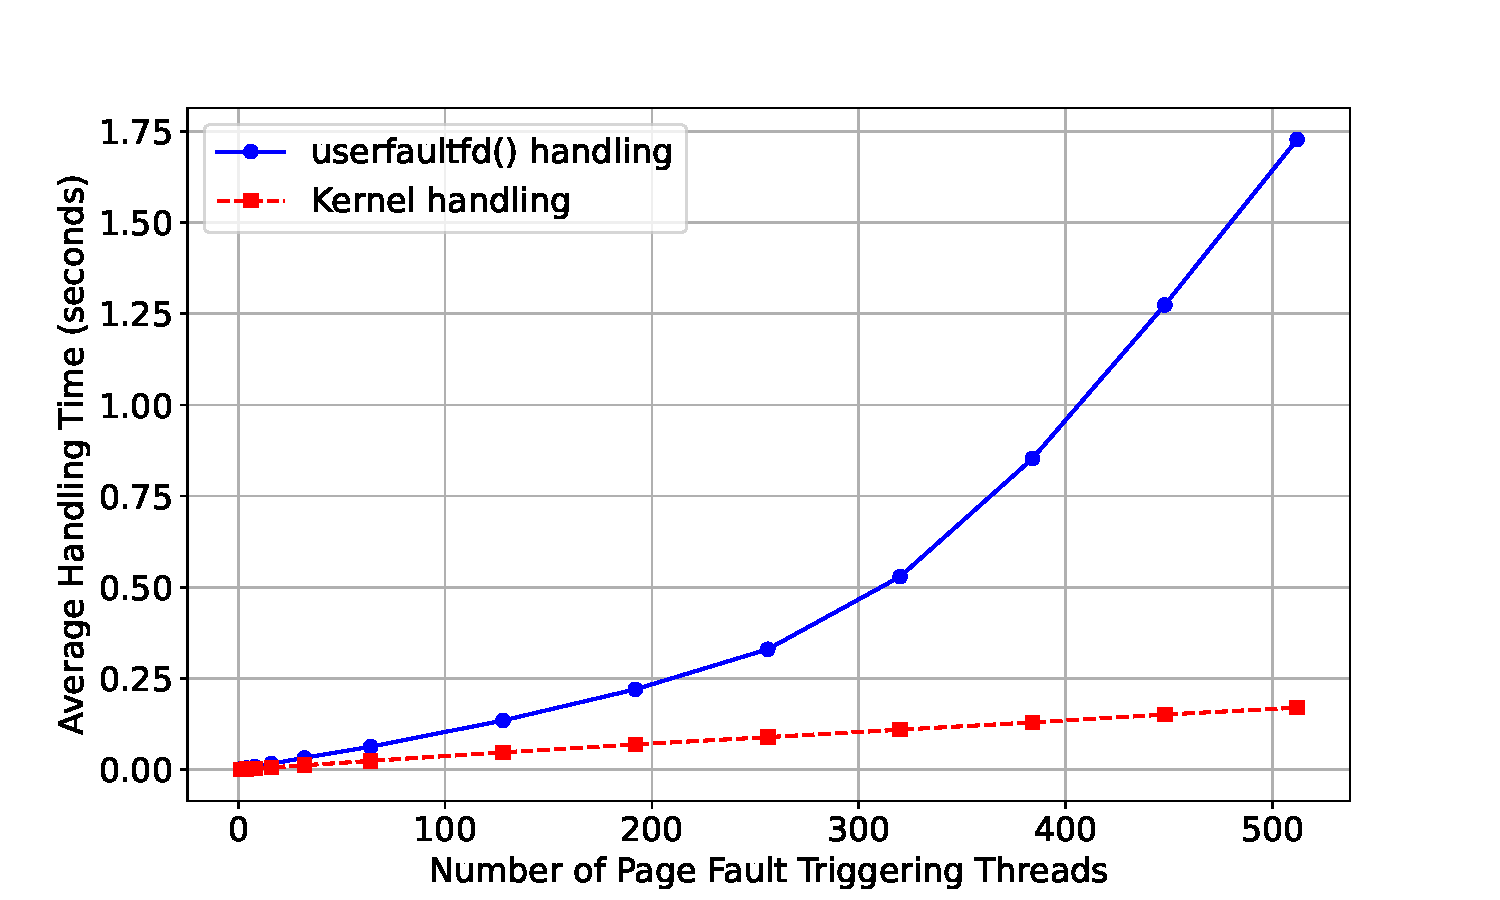
\includegraphics[clip,scale=0.33]{figures/motivation_scalability.pdf}
        \caption{To be added.}
        \label{fig:motivation-scalability} 
\end{figure}



% It does \texttt{copy\_from\_user}

\textbf{Security issue} \uffd might block the kernel\cite{uffd-blocking}, and is a common technique for kernel exploitation. For example, if the page fault handler choose to sleep (and nothing prevents it from doing that), the faulting thread will be stuck. This makes it easier to manipulate the execution order of process, and can be used to trigger race conditions on purpose. \teng{My point is, probably ebpf verifier can check for this?}

% No, eBPF programs cannot actively sleep like userspace programs can. However, they can call helper functions that can sleep, such as bpf_copy_from_user_stack. For example, a sleepable BPF program can call the bpf_copy_from_user_task helper when helper execution may be interrupted. However, the program doesn't have control over how long the helper function will sleep. 

Also, heap spraying (can ebpf solve this?)
https://etenal.me/archives/1336